\chapter{Modelado de la parte determinística \\ mediante Matching Pursuit}\label{capit:cap3}
\vspace{-2.0325ex}%
\noindent
\rule{\textwidth}{0.5pt}
\vspace{-5.5ex}% 
\newcommand{\pushline}{\Indp}% Indent puede ir o no :p


Este capítulo presenta una breve descripción del algoritmo iterativo \emph{Matching Pursuit} (MP), que descompone una señal en una combinación lineal de formas de onda elementales pertenecientes a un diccionario redundante de funciones. La compresión se realiza debido a que esta técnica es del tipo \emph{representación dispersa} de señales, es decir, mediante un número reducido de ondas se representan eventos cardiacos extrayendo una gran cantidad de su energía. De igual manera MP es conocido como un método de \emph{representación atómica}, dado que los bloques o diccionarios redundantes de funciones que se les conoce también como \emph{átomos}.

Se ha seleccionado un diccionario multi-bloques para la descomposición cuyos elementos son conocidos como \emph{átomos de Gabor} dada su alta correlación con los eventos cardiacos. 

\section{Representación dispersa de señales}

Una herramienta que ha demostrado ser eficiente en el análisis y representación de señales es la representación dispersa \cite[]{Gribonval2003,Gribonval2007,Elad2010,Mallat1993}. Varios de los procedimientos efectuados en el tratamiento de  señales de audio e imágenes como la transformación, compresión, \emph{de-noising}, separación de fuentes y otros métodos de codificación se han efectuado con eficiencia mediante esta técnica. A continuación se da una breve definición sobre la representación dispersa\footnote{Es conocida en Inglés como \emph{sparse representation.}} de señales.

El objetivo de la representación dispersa es encontrar una representación eficiente de un vector o señal $\mathbf{v} \in \mathcal{H}$, donde $\mathcal{H}=\mathbb{R}^{N}$

Una solución sencilla consistiría en tomar una base ortonormal $\Phi =\{ \phi_{1}, ..., \phi_{N}\}$ para $\mathcal{H}$ y usar los coeficientes de Fourier $\{\langle \mathbf{v},\phi_{k}\rangle\}_{k=1}^{N}$ para representar a $\mathbf{v}$. Esta respuesta es simple y funciona adecuadamente en muchos casos, sin embargo, también puede considerarse un tipo de expansión más general donde la base ortonormal es reemplazada por un diccionario adaptado formado desde $\mathcal{H}$. 

Un \textbf{diccionario} en $\mathcal{H} = \mathbb{R}^{N}$ es una familia de $K  > N$ vectores columna unitarios $\{\mathbf{g_{k}}\}$ que expande o genera a $\mathcal{H}$. En notación matricial se puede expresar como $\mathcal{\mathbf{D}} =[\mathbf{g_{1}},...,\mathbf{g_{K}}]$. 

Se entiende como una representación de $\mathbf{v}$ en $\mathcal{\mathbf{D}}$ un vector columna $\mathbf{\alpha} = (\alpha_{k}) \in \mathbb{R}^{K}$ tal que $\mathbf{v}=\mathcal{\mathbf{D}}\mathbf{\alpha}$. Es importante verificar que $K > N$, esto es, los vectores en $\mathcal{D}$ no son lo suficientemente independientes linealmente y la representación de $\mathbf{v}$ no es única. Se espera que para todas las representaciones posibles de $\mathbf{v}$ exista una \emph{muy reducida}, esto es, la representación con el menor número de coeficientes diferentes de cero. Este procedimiento es representado de manera sencilla en la Figura \ref{sparse_diagram}, donde se verifica que los pocos elementos distintos de cero del diccionario conforman la representación dispersa ideal de $\mathbf{v}$.
%================================
\begin{figure}[ht]
\begin{center}
\includegraphics[width=5.3in]
{sparse_diagram.pdf}
\end{center}
\par
\caption{Representación gráfica de una representación dispersa para una señal $\mathbf{v}$ desde un diccionario $\mathcal{\mathbf{D}}$.}
\label{sparse_diagram}
\end{figure}
%=======================================

Un compromiso que representa un problema en este proceso es el de encontrar todas las representaciones de $\mathbf{v}$ para encontrar las representaciones dispersas (procedimiento que lleva un largo tiempo) y entonces determinar si existe un conjunto único de representaciones dispersas. Varios tipos de diccionarios así como diversos procedimientos y modificaciones a los mismos se han analizado en la literatura para resolver esta encomienda en el menor tiempo posible \cite[]{Gribonval2007,Gribonval2003,Elad2010,RuizReyes2010}.

\section{Diccionarios tiempo-frecuencia}
Es a través de la transformada de Fourier como se describe una señal en términos de su contenido en frecuencia, lo cual se trata de una combinación de formas de onda ortogonales. Esta herramienta es la de uso más común en el análisis de señales en el dominio frecuencial debido a la facilidad que presentan las funciones senoidales siendo su base. 

Mediante una transformación por Fourier se lleva a cabo una proyección de una señal $x(t)$ sobre funciones base exponenciales complejas de frecuencia $\omega = 2\pi f$ :
%-----------------------
\begin{equation}\label{transFourier}
	X(\omega) = \int_{-\infty}^{\infty}x(t) e^{-i\omega t} dt,
\end{equation}
%-----------------------
donde $i=\sqrt{-1}$ y $X(\omega)$ es la \emph{transformada de Fourier} de la señal $x(t)$.

Sin embargo, no todas las señales son idealmente representadas por esta transformación, por ejemplo aquellas que presentan transitorios (cambios abruptos en frecuencia para instantes cortos de tiempo), cuyas irregularidades  requieren un análisis en tramos más consistentes. De esta manera surge la Transformada de Fourier de Tiempo Corto (STFT), la cual consiste en simplemente aplicar la transformada de Fourier a estructuras locales (segmentos con traslape) de la señal. 

En la STFT se incluye el uso de una \emph{ventana deslizante} $w(\tau - t)$ cuya localización es desplazada en el eje temporal, con lo que se proveerá un análisis en el plano tiempo frecuencia dado por la expresión \ref{STFT}:
%-----------------------
\begin{equation}\label{STFT}
	S(\omega,t) = \int_{-\infty}^{\infty}x(t)w(\tau-t) e^{-j\omega t} dt.
\end{equation}
%-----------------------
De aquí se deduce que el empleo de ondas bien concentradas\footnote{Que se conozcan completamente tanto en tiempo como frecuencia (finitas en ambos planos).} en el plano tiempo-frecuencia otorgarán una representación más adecuada en caso que la señal presente transitorios. El desarrollo de un modelo para el análisis o descomposición de señales se verá favorecido mediante la selección de los átomos óptimos, esto es que coincidan con las características básicas de la señal tanto en tiempo como en frecuencia \cite[]{Mallat1999}.

\subsection{Diccionario y átomos de Gabor}
El seleccionar un diccionario adecuado es una tarea fundamental en la descomposición y representación escasa de una señal. En la literatura se han propuesto diversos paquetes de ondas tiempo-frecuencia tales como ondeletas (\emph{wavelets}), paquetes de cosenos, transformadas de coseno discreto modificada y diccionarios de Gabor \cite[]{Wolfe2001}, etc. 

Estos bloques de ondas elementales  han sido probados en la reconstrucción de fonocardiogramas \cite[]{Nieblas2014}, obteniendo que los diccionarios de Gabor son los más adecuados para este propósito.

Los átomos de Gabor son ondas cosenoidales que se obtienen por la dilatación, traslación y modulación de una ventana madre $w(t)$, la cual generalmente toma valores reales y positivos además de tener una norma unitaria. La ecuación \eqref{gaborAtom} define esta forma de onda:
%-----------------------
\begin{equation}\label{gaborAtom}
	g_{\gamma}(t) = \frac{1}{\sqrt{s}}w\left(\frac{t-u}{s}\right) e^{i2\pi\xi(t-u)},
\end{equation}
%-----------------------
donde $w$ es una ventana gaussiana deslizante: $w(t)=\sqrt[4]{2}e^{-\pi t^{2}}$, la longitud de esta envolvente es controlada mediante la variable $s$, mientras que $u$ es un desplazamiento para especificar la localización temporal del átomo y $\xi$ es la frecuencia de modulación de la sinusoide. 
%================================
\begin{figure}[ht]
\begin{center}
\includegraphics[width=4.7in]
{atomo_gabor.eps}
\end{center}
\par
\caption{Forma de onda de un átomo de Gabor.}
\label{gaborWaveform}
\end{figure}
%=======================================

Se define entonces como diccionario o bloque de Gabor al conjunto constituido por las ondas previamente descritas: $\Gamma=\{\gamma_{m}\}_{m=1}^{K}$, donde cada uno de sus elementos se definen como $\gamma_{m}=(s_{m},u_{m},\xi_{m})$ . La Figura \ref{gaborWaveform} muestra la forma de onda de un átomo de Gabor. 

\subsection{Descomposiciones atómicas}
Las bases de ondeletas fueron las predecesoras a las bases de Fourier en la reconstrucción de señales. Pocos coeficientes son necesarios para representar las estructuras correspondientes a los transitorios locales de la señal mediante ondeletas \cite[]{Mallat1999}, constituyendo mediante este método un esquema de compresión.

La historia de la reconstrucción por ondeletas comienza con \cite{Haar1911}, quien propuso una función constante cuyas traslaciones y dilataciones constituyen una base ortonormal para la representación de señales. Esta ondeleta lleva su mismo nombre.

Posteriormente \cite{Gabor1946} propuso la descomposición de una señal sobre diccionarios de formas de onda elementales llamados átomos, los cuales tienen un esparcimiento mínimo en el plano tiempo-frecuencia. En efecto, a este método se le denomina descomposición atómica de señales. 

Para la reconstrucción de la señal se lleva a cabo la suma de los átomos tiempo-frecuencia seleccionados del diccionario. Es fundamental el hecho de entender que los diccionarios son bloques de formas de onda atómicos los cuales presenten elementos de características tiempo-frecuencia adaptados a las propiedades de la señal; la mejor representación de la señal es un problema complejo, dado que existen un sinfín de descomposiciones posibles \cite[]{Gribonval2007}. 

Sea una señal continua $x(t)$, cuya representación atómica en un conjunto de $K$ funciones $g_{m}(t)$ tiene la siguiente estructura:
%-----------------------
\begin{equation}\label{atomicDecomp}
	x(t) = \sum_{i=1}^{K}\alpha_{i}g_{i}(t),
\end{equation}
%-----------------------

donde los coeficientes $\alpha_{i}$ denotan la ponderación asociada a cada función átomo $g_{i}(t)$. También deberá asimilarse que la señal $x(t)$ es finita, para que su energía sea adecuadamente representada tanto en tiempo como en frecuencia (esta representación también puede realizarse con una señal discreta $x(n)$ finita de $N$ elementos). 

La selección de funciones elementales o átomos que mejor aproximan a $x(t)$ así como el cálculo de los coeficientes $\alpha_{i}$ puede realizarse mediante diversos métodos \cite[]{Nieblas2014}, en este caso se ha seleccionado el algoritmo iterativo \emph{Matching Pursuit} \cite[]{Mallat1993}.

\subsection{Principio de incertidumbre de Heisenberg}

Es importante en una descomposición atómica el conocer la concentración de energía de las ondas tiempo-frecuencia empleadas, lo cual garantizará una buena reconstrucción de la señal tratada \cite[]{Mallat1999}. En este caso, los átomos de Gabor son construidos por la traslación en tiempo y frecuencia de una ventana $g$:
%-----------------------
\begin{equation}\label{gaborAtom2}
	g_{u,\xi}(t) = g(t-u)e^{i\xi t},
\end{equation}
%-----------------------
donde $u$ y $\xi$ son las traslaciones o desplazamientos en tiempo y frecuencia correspondientemente.

La energía de $g_{u,\xi}$ se concentra en la vecindad de $u$ sobre un intervalo de tiempo de $\sigma_{t}$. La transformada de Fourier $\widehat{G}$ se traslada mendiante $\xi$ por medio de:
%-----------------------
\begin{equation}\label{gaborAtomTF}
	g_{u,\xi}(\omega) = g(\omega-\xi)e^{-iu(\omega-\xi)}.
\end{equation}
%-----------------------
La energía de $\widehat{g}_{u,\xi}$ se localiza sobre la frecuencia $\xi$ en un intervalo de tamaño $\sigma_{\omega}$. Para el plano tiempo-frecuencia $(t,\omega)$ la energía del átomo ${g}_{u,\xi}$ se representa simbólicamente por un \emph{rectángulo de Heisenberg}, el cual está centrado en $(u,\xi)$ y tiene un largo de duración de tiempo $\sigma_{t}$ y un ancho en frecuencia $\sigma_{\omega}$. El principio de incertidumbre de Heiseberg satisface la desigualdad siguiente:
%-----------------------
\begin{equation}\label{Heis}
	\sigma_{t} \sigma_{\omega} \geq \frac{1}{2}.
\end{equation}
%-----------------------
El área del rectángulo de Heisenberg $\sigma_{t}\sigma_{\omega}$ es mínima para una $g$ tipo gaussiana, en cuyo caso hemos visto que los átomos $g_{u,\xi}$ son llamados funciones de Gabor. La Figura \ref{HeisBoxes} otorga una descripción gráfica en cajas de Heisenberg de dos átomos tiempo-frecuencia, cuya estructura gaussiana favorece el soporte en ambos planos.
%================================
\begin{figure}[ht]
\begin{center}
\includegraphics[width=4.7 in]
{gabor_boxes.pdf}
\end{center}
\par
\caption{Representación de dos átomos tiempo-frecuencia en cajas de Heisenberg.}
\label{HeisBoxes}
\end{figure}
%=======================================

\section{Descomposición de fonocardiogramas mediante Matching Pursuit (MP)}
 Tras con anterioridad haber descrito la importancia de las descomposiciones atómicas y la representación escasa de señales por medio de diccionarios tiempo-frecuencia (en específico los definidos por Gabor) es conveniente mencionar un algoritmo que conjunta estas técnicas como lo es Matching Pursuit \cite[]{Mallat1993}. 
 
 Se ha presentado también MP en la literatura como un auxiliar muy completo en el análisis de fonocardiogramas, debido a que la mayor cantidad de la energía de éstos puede concentrarse por medio de este método en una representación de un número iterativo deseado de formas de onda elementales \cite[]{Zhang1998a,Zhang1998b,wang04,Sava1998}. Esto es, la cantidad de iteraciones deseada es proporcional al número de átomos de la representación y cuan mayor sea se preservará en efecto mayor energía en la reconstrucción.
 
Matching Pursuit es un algoritmo codicioso (\emph{greedy}) debido a que en cada iteración sigue extrayendo energía a la señal analizada, resolviendo el problema de la mejor representación analizado al inicio de este capítulo mediante la realización del máximo absoluto del producto interno (también considerado como \emph{correlación} en este caso). Esta operación garantiza el encontrar los átomos que mejor coincidan (\emph{best-match}) con la estructura local de la señal en la iteración correspondiente. 

La combinación lineal de formas de onda elementales, representación escasa o descomposición atómica de una señal $x(t)$ mediante MP está dada por la expresión \eqref{MatchingPursuit}:
%-----------------------
\begin{equation}\label{MatchingPursuit}
	x(t) = \sum_{m=1}^{M} \alpha_{m} \cdot g_{\gamma_{m}}(t) + R_{M}(t),
\end{equation}
%-----------------------
donde $M$ es el número de iteraciones ó átomos deseado en la descomposición, $g_{\gamma_{m}(t)}$ es el átomo $m$-ésimo óptimo del bloque o diccionario (esto es, $\gamma \in \Gamma$), $\alpha_{m}$ el factor de ponderación y $R_{M}(t)$ un término residual surgido de la diferencia entre la señal y el átomo ponderado después de la m-ésima iteración. 

Por medio del Algoritmo \ref{MP} se observan los procedimientos correspondientes a la obtención de dichos términos, donde la relación señal a ruido (Signal to Noise Ratio, SNR) es obtenida como el cociente de la energía de la señal reconstruida por la suma de los átomos ponderados entre la energía de la señal residual.

% ++++++++++++++++++++++++++++++++++++
\begin{algorithm}
\begin{algorithmic}
\REQUIRE $x(t)$, $\mathcal{D}= \{ g_{\gamma}(t), \gamma \in \Gamma \}$
\ENSURE $\alpha_{m}, g_{\gamma_{m}}(t)$
\STATE {$R=x(t)$}
\STATE {$\alpha_{m} = 0$}
\REPEAT 
	\STATE{$g_{\gamma_{m}} = \arg\max_{\gamma \in \Gamma} \lvert \langle R,g_{\gamma} \rangle \rvert$}
	 \STATE{$\alpha_{m} = \langle R,g_{\gamma} \rangle$}
	 \STATE{$R= R-\alpha_{m}\cdot g_{\gamma_{m}}$}
\UNTIL {se alcance la cantidad de iteraciones o SNR deseadas.}
\end{algorithmic}
\caption {Matching Pursuit}
\label{MP}
\end{algorithm}
%++++++++++++++++++++++++++++++++++++

Observando la forma de onda de los átomos de Gabor puede deducirse su alta correlación con los eventos cardíacos, por lo cual solamente estas partes de la señal son adecuadamente modeladas y reconstruidas mediante Matching Pursuit y diccionarios de este tipo logrando una compresión. 

La \emph{segmentación} es el primer paso para el análisis del fonocardiograma, de esta manera se extraerán solamente los sonidos cardiacos principales y patologías para realizar su descomposición. Este proceso puede realizarse de manera manual o automática por medio de algún algoritmo \cite[]{Nieblas2013}.

Durante la segmentación se detectan los tiempos de inicio \emph{(on-set)} y final \emph{(off-set)} de algún sonido normal o patología cardiaca. Estos instantes de tiempo ayudan a diferenciar las partes del fonocardiograma que son silencio y las que se consideran evento.

\subsection{Criterios en la descomposción de fonocardiogramas por MP}

A pesar de tener una reconstrucción aceptable en las señales de fonocardiograma tras representarlas en los átomos seleccionados desde Matching Pursuit el 100\% de la energía realmente nunca es alcanzado, se tiene un comportamiento asintótico entre ésta variable y el número de iteraciones. 

Esto se observa con detenimiento en la Figura \ref{porcentEnergia}, para lo cual se ha hecho un acercamiento en la parte donde parece haberse restablecido el total de la energía (de las 21 a las 30 iteraciones). 

%================================
\begin{figure}[h!]
\begin{center}
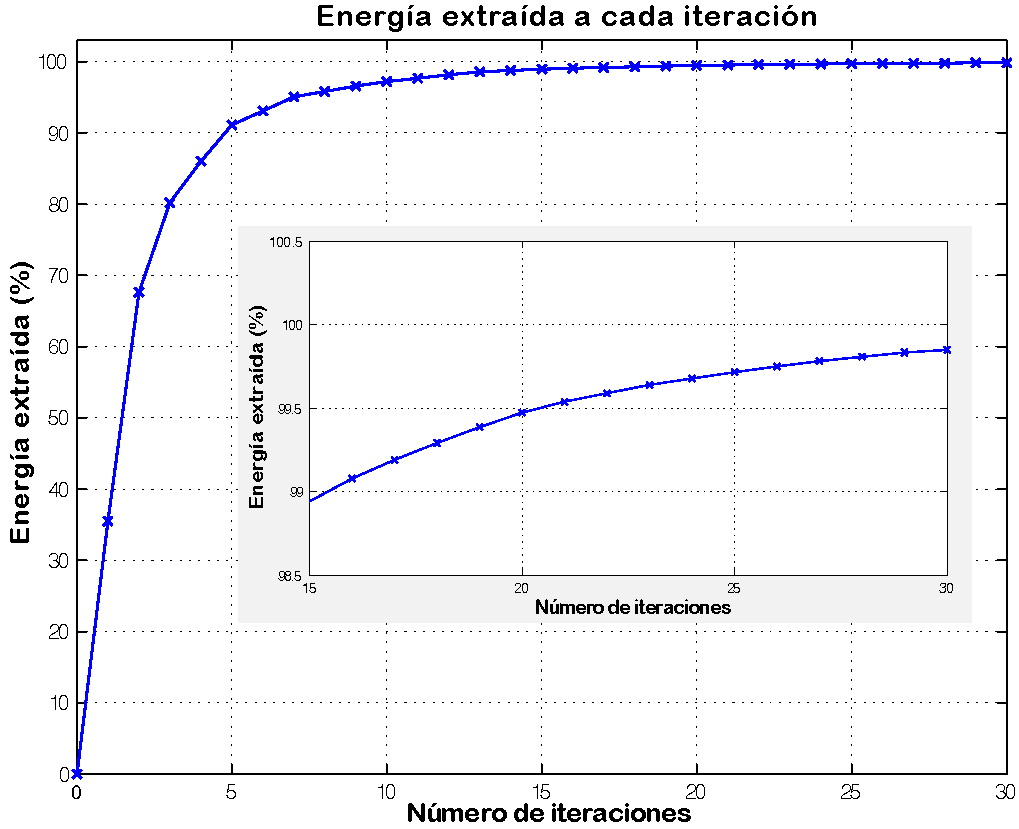
\includegraphics[width=3.5in]
{perfil_energia_extraida.pdf}
\end{center}
\par
\caption{Porcentaje de energía recobrada/extraída tras cada iteración realizada en Matching Pursuit. Se observa en el acercamiento a la gráfica que tras $M=30$ iteraciones realmente no se retiene el total de la energía.}
\label{porcentEnergia}
\end{figure}
%=======================================

Dado este comportamiento, en este trabajo se ha decidido representar mediante MP un 99\% de la energía de la señal, preservando el 1\% restante en la señal residual $R_{M}(t)$. Este residuo tiene correlación mucho más baja con respecto a las ondas de Gabor que el evento cardiaco inicial, que al igual que los silencios aún son perceptibles al oído humano debido al comportamiento logarítmico de este órgano natural receptor \cite[]{Smith1999}. 
 
 En la Figura \ref{eventoRecons} se ha realizado la reconstrucción de un evento cardíaco s1 con 10 iteraciones, cantidad necesaria para representar en un 99 \% su energía. Se muestra la forma de onda temporal de la señal original, el residual y la señal reconstruida, así como la representación en el plano tiempo-frecuencia en cajas de Heisenberg de los átomos necesarios para la descomposición. 
%================================
\begin{figure}[ht]
\begin{center}
\includegraphics[width = 6.8 in]
{eventoRecons.eps}
\end{center}
\par
\caption{Forma de onda temporal y gráfica en el plano tiempo-frecuencia en la reconstrucción de un evento cardiaco s1.}
\label{eventoRecons}
\end{figure}
%=======================================

La señal residual se modelará con técnicas de predicción lineal (LPC), presentadas en el siguiente capítulo. Esta señal se considera como la parte \emph{estocástica} del códec.

